\begin{frame}{Les dates}
  Quelle est date aujourd'hui? \underline{\uncover<2->{le 30 août}} \\
  \vspace{0.2cm}
  \uncover<3->{
    Quelle est la date de chaque fête? \\
    \tinygloss{What is the date of each holiday?}
    \begin{columns}
      \column{0.6\textwidth}
        \small
        \begin{enumerate}
          \item le jour de l'An $\to$ \underline{\uncover<4->{le 1er janvier}}
          \item Noël $\to$ \underline{\uncover<6->{le 25 décembre}}
          \item l'indépendance américaine
          \item[$\to$] \underline{\uncover<8->{le 4 juillet}}
          \item le Juneteenth $\to$ \underline{\uncover<10->{le 19 juin}}
          \item la journée des anciens combattants \gloss{veterans}
          \item[$\to$] \underline{\uncover<12->{le 11 novembre}}
        \end{enumerate}
      \column{0.4\textwidth}
        \begin{minipage}[c][0.6\textheight]{\linewidth}
          \begin{center}
            \only<3-4>{
              
\includegraphics[scale=0.16]{nouvel_an.jpg}
            }
            \only<5-6>{
              
\includegraphics[scale=0.07]{noel.jpg}
            }
            \only<7-8>{
              \includegraphics[scale=0.2]{indépendance.jpg}
            }
            \only<9-10>{
              
\includegraphics[scale=0.11]{juneteenth.jpg}
            }
            \only<11-12>{
              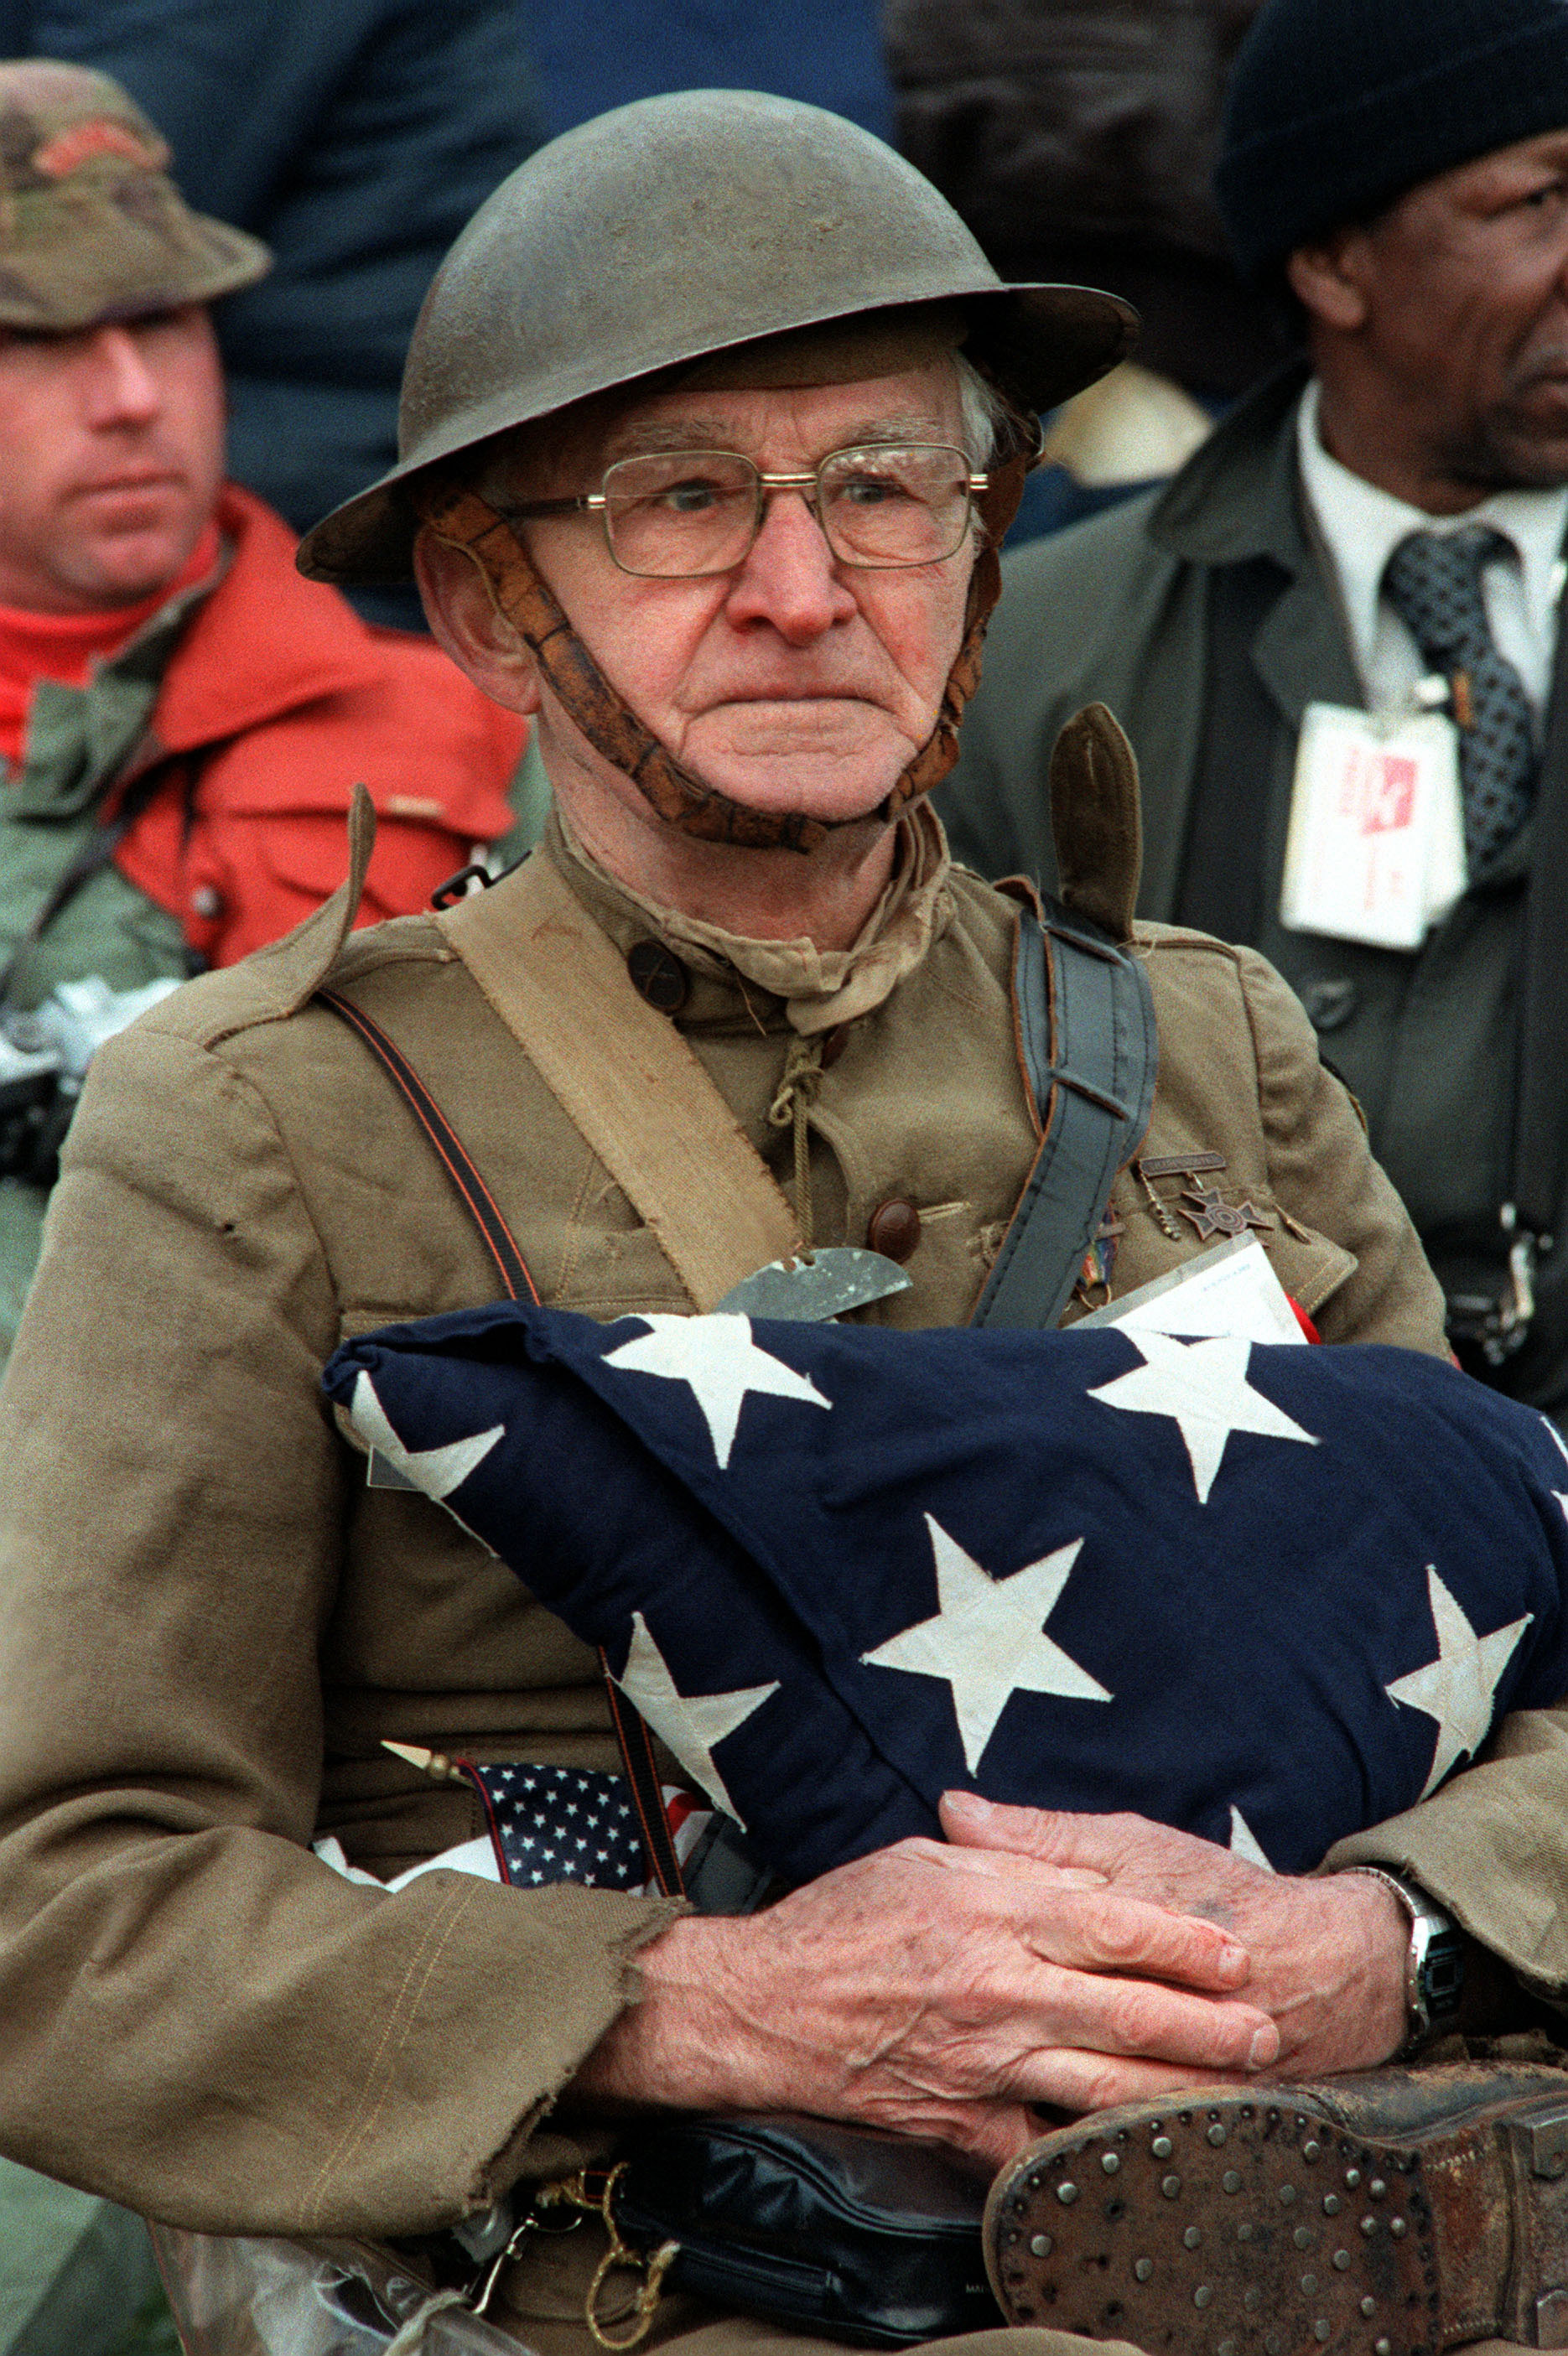
\includegraphics[scale=0.2]{veteran.jpg}
            }
          \end{center}
        \end{minipage}
    \end{columns}
  }
\end{frame}